\documentclass[11pt,compress,t,notes=noshow, xcolor=table]{beamer}

\usepackage[]{graphicx}\usepackage[]{color}
% maxwidth is the original width if it is less than linewidth
% otherwise use linewidth (to make sure the graphics do not exceed the margin)
\makeatletter
\def\maxwidth{ %
  \ifdim\Gin@nat@width>\linewidth
    \linewidth
  \else
    \Gin@nat@width
  \fi
}
\makeatother

\definecolor{fgcolor}{rgb}{0.345, 0.345, 0.345}
\newcommand{\hlnum}[1]{\textcolor[rgb]{0.686,0.059,0.569}{#1}}%
\newcommand{\hlstr}[1]{\textcolor[rgb]{0.192,0.494,0.8}{#1}}%
\newcommand{\hlcom}[1]{\textcolor[rgb]{0.678,0.584,0.686}{\textit{#1}}}%
\newcommand{\hlopt}[1]{\textcolor[rgb]{0,0,0}{#1}}%
\newcommand{\hlstd}[1]{\textcolor[rgb]{0.345,0.345,0.345}{#1}}%
\newcommand{\hlkwa}[1]{\textcolor[rgb]{0.161,0.373,0.58}{\textbf{#1}}}%
\newcommand{\hlkwb}[1]{\textcolor[rgb]{0.69,0.353,0.396}{#1}}%
\newcommand{\hlkwc}[1]{\textcolor[rgb]{0.333,0.667,0.333}{#1}}%
\newcommand{\hlkwd}[1]{\textcolor[rgb]{0.737,0.353,0.396}{\textbf{#1}}}%
\let\hlipl\hlkwb

\usepackage{framed}
\makeatletter
\newenvironment{kframe}{%
 \def\at@end@of@kframe{}%
 \ifinner\ifhmode%
  \def\at@end@of@kframe{\end{minipage}}%
  \begin{minipage}{\columnwidth}%
 \fi\fi%
 \def\FrameCommand##1{\hskip\@totalleftmargin \hskip-\fboxsep
 \colorbox{shadecolor}{##1}\hskip-\fboxsep
     % There is no \\@totalrightmargin, so:
     \hskip-\linewidth \hskip-\@totalleftmargin \hskip\columnwidth}%
 \MakeFramed {\advance\hsize-\width
   \@totalleftmargin\z@ \linewidth\hsize
   \@setminipage}}%
 {\par\unskip\endMakeFramed%
 \at@end@of@kframe}
\makeatother

\definecolor{shadecolor}{rgb}{.97, .97, .97}
\definecolor{messagecolor}{rgb}{0, 0, 0}
\definecolor{warningcolor}{rgb}{1, 0, 1}
\definecolor{errorcolor}{rgb}{1, 0, 0}
\newenvironment{knitrout}{}{} % an empty environment to be redefined in TeX

\usepackage{alltt}
\newcommand{\SweaveOpts}[1]{}  % do not interfere with LaTeX
\newcommand{\SweaveInput}[1]{} % because they are not real TeX commands
\newcommand{\Sexpr}[1]{}       % will only be parsed by R
\newcommand{\xmark}{\ding{55}}%


\usepackage[english]{babel}
\usepackage[utf8]{inputenc}

\usepackage{dsfont}
\usepackage{verbatim}
\usepackage{amsmath}
\usepackage{amsfonts}
\usepackage{amssymb}
\usepackage{bm}
\usepackage{csquotes}
\usepackage{multirow}
\usepackage{longtable}
\usepackage{booktabs}
\usepackage{enumerate}
\usepackage[absolute,overlay]{textpos}
\usepackage{psfrag}
\usepackage{algorithm}
\usepackage{algpseudocode}
\usepackage{eqnarray}
\usepackage{arydshln}
\usepackage{tabularx}
\usepackage{placeins}
\usepackage{tikz}
\usepackage{setspace}
\usepackage{colortbl}
\usepackage{mathtools}
\usepackage{wrapfig}
\usepackage{bm}
\usepackage{amsmath}
\usepackage{pifont}

\usetikzlibrary{shapes,arrows,automata,positioning,calc,chains,trees, shadows}
\tikzset{
  %Define standard arrow tip
  >=stealth',
  %Define style for boxes
  punkt/.style={
    rectangle,
    rounded corners,
    draw=black, very thick,
    text width=6.5em,
    minimum height=2em,
    text centered},
  % Define arrow style
  pil/.style={
    ->,
    thick,
    shorten <=2pt,
    shorten >=2pt,}
}

\usepackage{subfig}

% Defines macros and environments
\usepackage{../../style/lmu-lecture}


\let\code=\texttt
\let\proglang=\textsf

\setkeys{Gin}{width=0.9\textwidth}

\setbeamertemplate{frametitle}{\expandafter\uppercase\expandafter\insertframetitle}


% basic latex stuff
\newcommand{\pkg}[1]{{\fontseries{b}\selectfont #1}} %fontstyle for R packages
\newcommand{\lz}{\vspace{0.5cm}} %vertical space
\newcommand{\dlz}{\vspace{1cm}} %double vertical space
\newcommand{\oneliner}[1] % Oneliner for important statements
{\begin{block}{}\begin{center}\begin{Large}#1\end{Large}\end{center}\end{block}}






%\newcommand{\titlefigure}{} MISSING
\newcommand{\learninggoals}{
  \item \textcolor{blue}{XXXXXXXXXXXXXXXX}
  \item \textcolor{blue}{XXXXXXXXXXXXXXXX}
}



\title{Introduction to Machine Learning}
% \author{Bernd Bischl, Christoph Molnar, Daniel Schalk, Fabian Scheipl}
\institute{\href{https://compstat-lmu.github.io/lecture_i2ml/}{compstat-lmu.github.io/lecture\_i2ml}}
\date{}

\setbeamertemplate{frametitle}{\expandafter\uppercase\expandafter\insertframetitle}



\begin{document}


\lecturechapter{Random Forest: OOB error estimate}
\lecture{Introduction to Machine Learning}
\sloppy



\begin{vbframe}{OOB error for Random Forests}
In section 2 / slide 7 we saw the following description about the estimation of the OOB error in random forests:
\begin{center}
%https://docs.google.com/presentation/d/16gg9PqtEV_Ii_ZBw0zA9GdUIled-6OVkoqArX1ouTmo/edit#slide=id.g4193e2316a_0_68
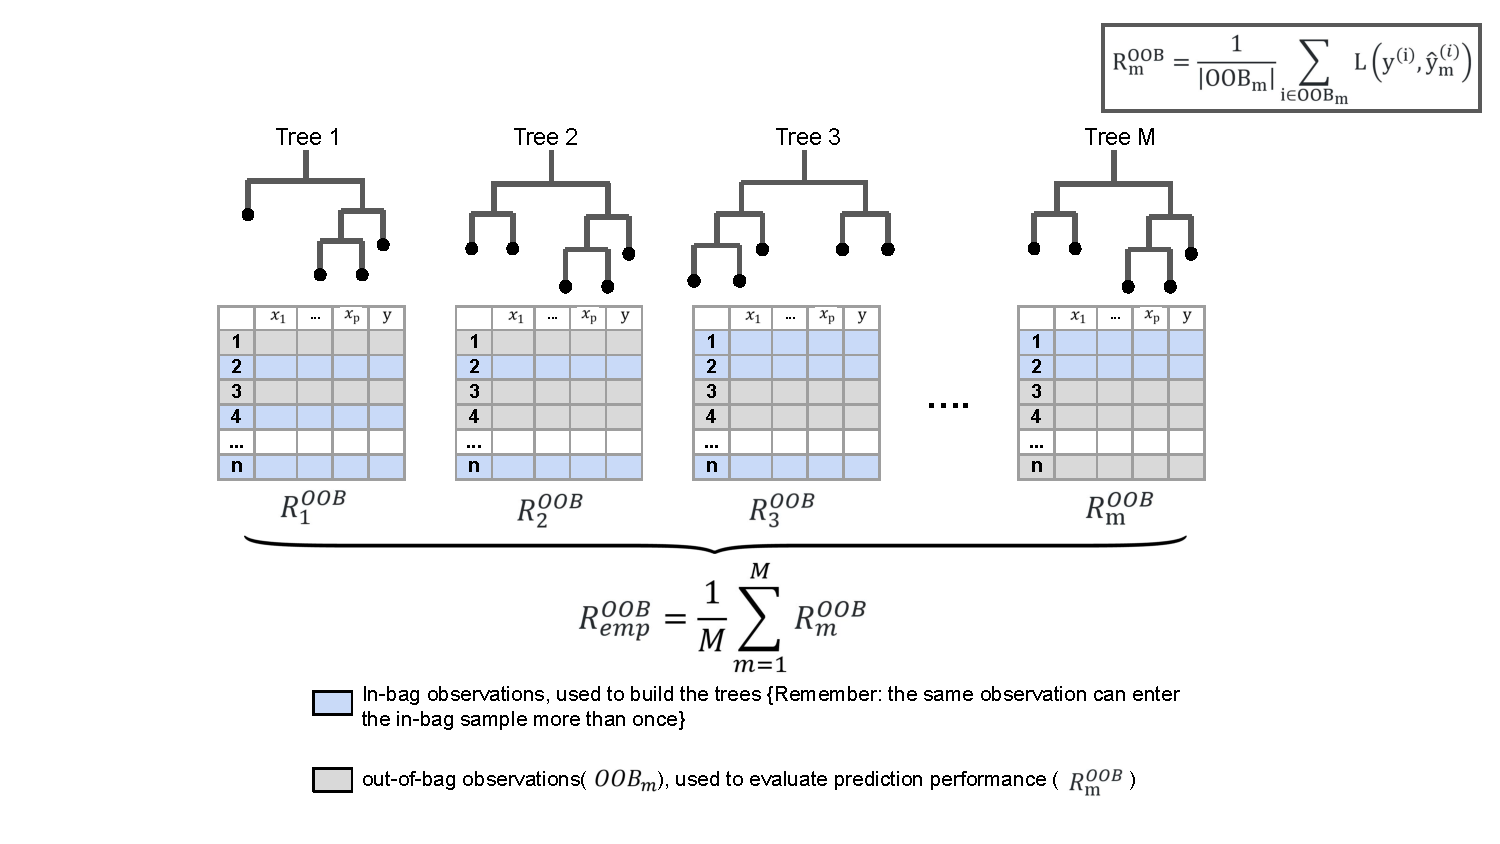
\includegraphics[width=0.65\textwidth]{figure_man/rF_oob_error_new.pdf}
\end{center}

\begin{itemize}
  \item OOB size: $P(\text{not drawn}) = \left(1 - \frac{1}{n}\right)^n \ \stackrel{n \to \infty}{\longrightarrow} \ \frac{1}{e} \approx 0.37$
  \item Predict all observations with trees that didn't use them for training and compute average loss of these predictions
  \item Similar to 3-CV, can be used for a quick model selection
\end{itemize}


\end{vbframe}


\begin{vbframe}{OOB error for Random Forests}
\begin{itemize}
\item This description is not entirely correct. In the following, we will see the correct description to estimate the OOB error. 
\item Each observation is passed down every  tree where this observation is an out-of bag-observation. On average, each observation is OOB in 37\% of the trees. 
\item In the next step (the aggregation step), we average the predictions from all of these trees (in regression setting). In a classification setting, we simply calculate the relative frequencies of all possible classes. 
\item The result from this aggregation step is then used as the prediction for the respective observation. For each observation, the loss function is evaluated. 
\item Finally, the generalization error is estimated as the average of the single losses.  
\end{itemize}
\end{vbframe}


\begin{vbframe}{OOB error for Random Forests}
\begin{itemize}
\item The original description (compare slide 1) implied that the loss function is applied to the predictions from the single trees directly. 
\item This is not true, the loss function is applied to the aggregation from the single trees. 
\item We denote the set of trees where observation $i$ is out-of-bag by $OOB_i$ and the predictions for observation $i$ from a single tree $j$ by $\hat y_i^{(j)}$.
\item In a regression setting, the predicted target value for observation $i$ can easily be derived by $\hat y^{oob}_{i} = \dfrac{1}{|OOB_i|}\sum\limits_{j\in OOB_i} \hat y_i^{(j)}$
\item The generalization error is then estimated via $$R_{emp}^{oob} = \dfrac 1n \sum_{i=1}^n L(y_i, \hat  y^{oob}_{i})$$
\end{itemize}
\end{vbframe}


\begin{vbframe}{Feature importance for Random Forests}
\begin{itemize}
\item The same holds true for the description of the variable importance in section 3 / slide 4.
\begin{center}
% FIGURE SOURCE: https://docs.google.com/presentation/d/16gg9PqtEV_Ii_ZBw0zA9GdUIled-6OVkoqArX1ouTmo/edit#slide=id.p
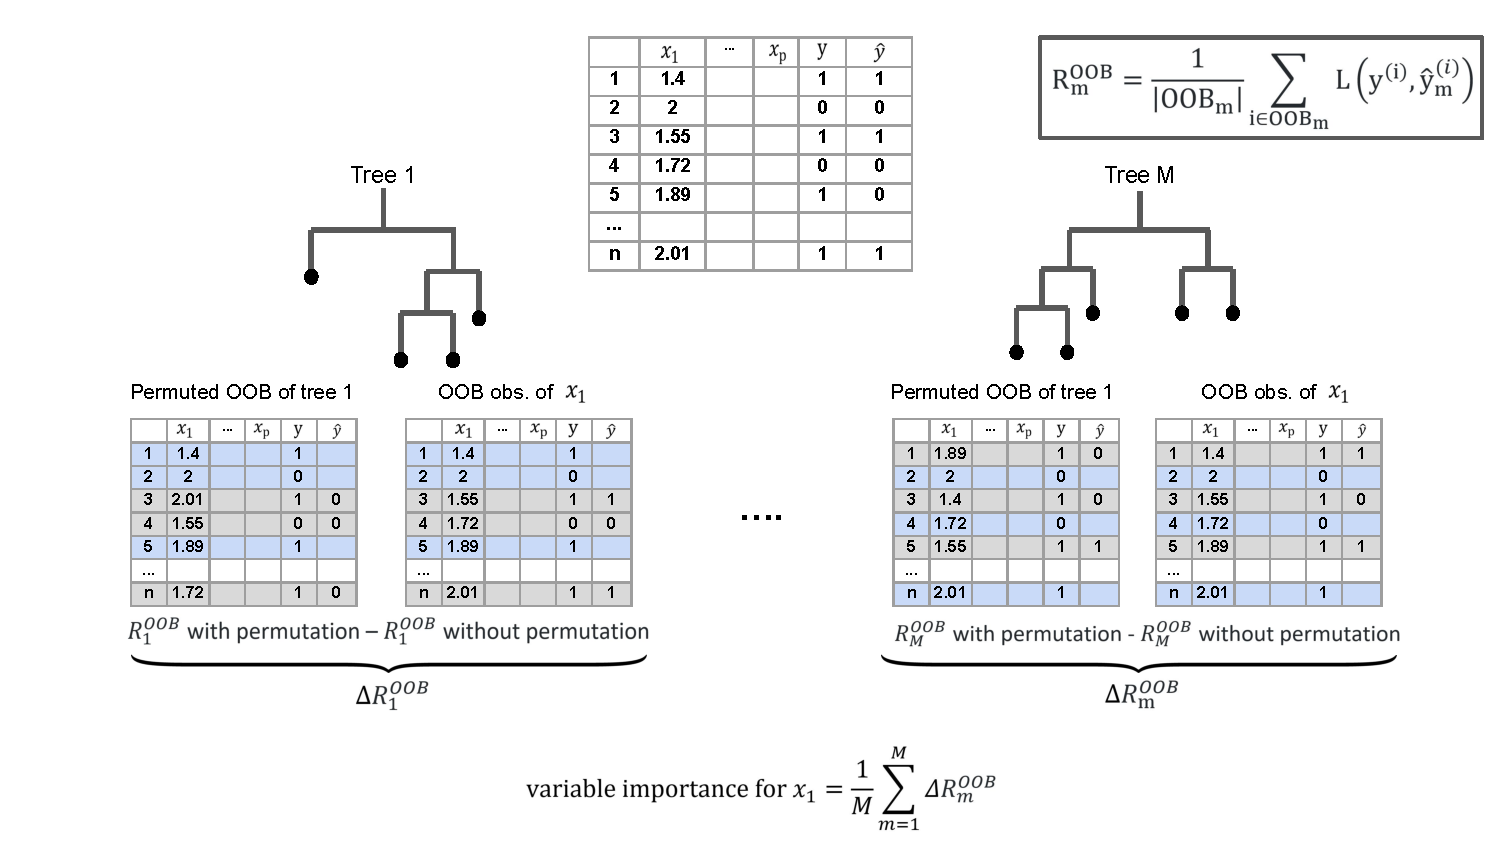
\includegraphics[width = 8cm]{figure_man/rF_varImp_permutation_new.pdf}
\end{center}
\item Again, (contrary to the schematic description above) it is \textbf{not} true that the loss function is applied to each prediction of the single trees  individually, but is applied to the aggregation of these predictions. 
\end{itemize}
\end{vbframe}

\endlecture
\end{document}
